
\begin{figure}
    \centering
    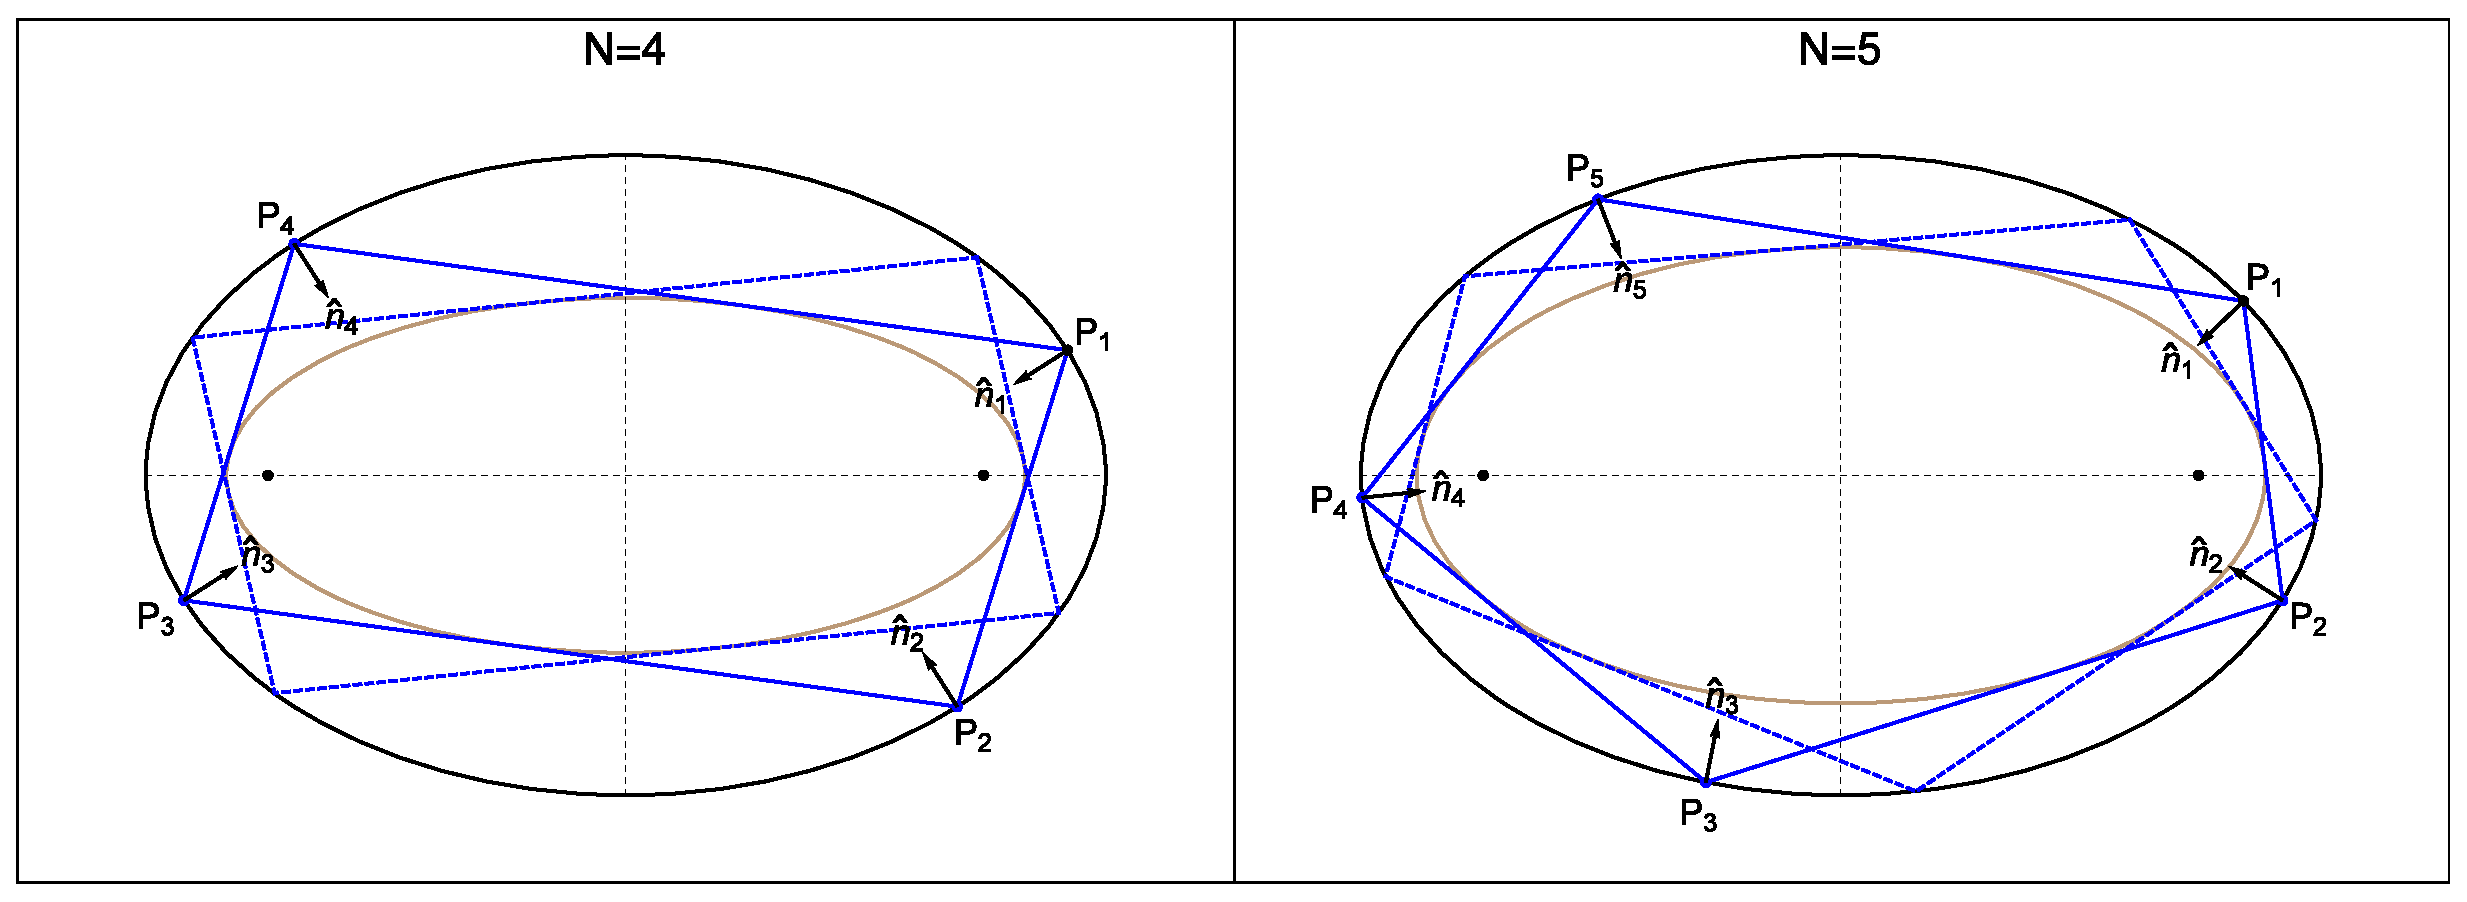
\includegraphics[scale=0.35]{pics_proposal/0000_n4n5.eps}
    \caption{Bilhar Elíptico e (4,5)-órbitas periódicas (azul) . Em todo vértice o vetor normal $\hat{n}_i$ bissecta os segmentos   de órbitas bilhares  $P_{i-1} P_{i}$ e $P_i P_{i+1}$ que são tangentes à cáustica (marrom). Uma segunda órbita também é mostrada (azul pontilhado). Note que o perímetro é conservado sobre toda a família de N-periódicas.   \href{https://youtu.be/Y3q35DObfZU}{Video}}
    \label{fig:n4n5}
\end{figure}
 \newpage
\begin{enumerate}
    \item \textbf{Nível}: Introdutório.
    \item \textbf{Duração}: 5 aulas de 45 minutos.
    \item \textbf{Descrição detalhada}: 
    \begin{itemize}
        \item \textbf{Objetivos}: Introdução à geometria dos bilhares elípticos \cite{darboux1917,lebesgue1942,rozikov2018,sergei91}, tema de grande influência na matemática dos últimos 200 anos. Divulgar novos invariantes ali manifestados, o método experimental de descoberta, e esboçar algumas provas.
        \item \textbf{Público-Alvo}: aluno(a)s de graduação ou pós, professores, ou quaisquer interessado(a)s em conhecer novas e belas propriedades do bilhar elíptico encontradas experimentalmente.
        \item \textbf{Conteúdo}: Geometria do bilhar elíptico, porisma de Poncelet e condições de Cayley \cite{dragovic11}, loci de centros triangulares \cite{etc} sobre a fam\'ilia de 3-periódicas, órbitas auto-intersectadas, polígonos inversivos, outras famílias Ponceletianas. Exemplificar alguns fenômenos por vídeos \cite{reznik2020-youtube} e/ou ferramenta interativa \cite{reznik2020-app}.
        \item \textbf{Monitoria}: co-autores e/ou alunos de iniciação científica farão revezamento.
        \end{itemize}
        \item \textbf{Distribuição de capítulos}:
        \begin{itemize}
            \item  Capítulo 1: Propriedades focais das cônicas \cite{akopyan2007-conics,berger1987,darboux1917,lebesgue1942}. Família confocal de cônicas. Relações entre elipses e triângulos (inscritos e circunscritos). 
            Introdução ao bilhar elíptico e ao porisma de Poncelet.  Condições de Cayley.
             Exercícios e projetos.
            
            \item Capítulo 2:
             Centros triangulares (incentro, baricentro, circuncentro, ortocentro, mittenpunkt etc). Coordenadas trilineares e baricêntricas no plano. Propriedades básicas de alguns  centros triangulares  \cite{ coxeter67,   kimberling98} e triângulos derivados (pedal, tangente, excentral etc).
            Loci e Invariantes Básicas: Loci elípticos de centros triangulares, soma de cossenos, razão de áreas, potência de um ponto em relação a um círculo.  Método experimental e algebro-computacional \cite{  garcia2019-incenter, garcia2020-ellipses, garcia2020-new-properties}.
            Exercícios e projetos.
            %Sketch das provas já publicadas. \cite{akopyan2020-invariants,bialy2020-invariants,caliz2020-area-product}.
            
            \item Capítulo 3: N-periodicas auto-intersectadas, condições de Birkhoff \cite{birkhoff66}. \textit{Tour } de N-periódicas auto-intersectadas. Exercícios e projetos.
            
            \item Capítulo 4: Inversão com respeito a um círculo. O talentoso polígono foco-inversivo, seus invariantes e propriedades. Exceções em invariantes. Exercícios e projetos.
            %Conexão com a transformação de Moebius.
            \item Capítulo 5: Alguns invariantes em outras famílias Ponceletianas, e.g., homotética, porística, com incírculo, circumcírculo  etc. Exercícios e projetos.
            
               \item Capítulo 6:  Tópicos de bilhares em curvas convexas e polígonos. Uma conexão rápida com vários outros ramos da matemática, contextualizando os problemas em aberto. Resenha de problemas de investigação no contexto de bilhares.
               
        \end{itemize}
        \item Pré-requisitos: conhecimentos básicos de Construções Geométricas,  Geometria Analítica, Álgebra Linear e Cálculo Diferencial.
        
        \item Número de páginas: Uma estimativa preliminar é de 120 páginas com muitas figuras ilustrando as propriedades geométricas observadas em experimentos computacionais no  bilhar elíptico e links para vídeos no youtube.
        
        \item Outras informações: a boa recepção da nossa palestra de divulgação  ``Aventuras com Triângulos e Bilhares'' ministrada no 32$^{\underline{o}}$  CBM do IMPA (2019) \cite{reznik2019-impa-talk,reznik2019-impa-article} além de nossas publicações em 2020  \cite{reznik2020-intelligencer,garcia2020-ellipses,garcia2020-new-properties,reznik2020-ballet,reznik2021-circum,reznik2021-fifty-invariants,garcia2020-similarity-I,garcia2020-steiner,reznik2020-similarityII,garcia2020-self-intersected,reznik2020-n3-focus-inversive}, nos motivou em propor esse curso com novos resultados e mais detalhes das técnicas utilizadas.
        \vskip .5cm
       Anexo segue artigo aceito para publicação na revista Amer. Math. Monthly ilustrando alguns resultados obtidos pelos proponentes. Também anexamos o artigo publicado na revista Math. Intelligencer.
        
\end{enumerate}





